
\section{Resultate}
\label{Resultate}

In diesem Kapitel werden die Resultate der Arbeit präsentiert und mit den im Kapitel \ref{Stand der Technik:Aktuelle Situation} vorgestellten bestehenden Berechnungsmethoden verglichen.
Die technische Beschreibung zur Implementation befindet sich im Teil \ref{SW-Projektdokumentation} Kapitel \ref{Implementation}.

\subsection{Zielerreichung}
\label{Resultate:Zielerreichung}

In der Evaluations-Phase (Kap. \ref{Stand der Technik}) wurden bestehende Ansätze zur Berechnung von \acs{ÖV}-Güteklassen analysiert und verglichen.
Es zeigte sich, dass die Methoden auf einer alten Norm aufbauen, die von einigen Kantonen etwas erweitert wurden.
Für die Berechnung der ganzen Schweiz gibt es aber keine Spezifikation, die moderne Analysen wie die Berücksichtigung des Strassennetzes vorsehen.

Unter Zuhilfenahme der Berechnungsmethodik des Kanton Graubündens erstellten wir anschliessend eine eigene Spezifikation, die "`\acs{ÖV}-Güteklassen 2018"'.
Dabei haben wir neben einer genaueren Ermittlung der Erreichbarkeit (Kap. \ref{Verbesserungsmöglichkeiten:Ermittlung der Erreichbarkeit der Haltestelle}) und die Berücksichtigung des Terrains auch Punkte konkretisiert, die in bisherigen Methoden nicht genau spezifiziert sind, wie etwa die Berechnung des Kursintervalls (Kap. \ref{Verbesserungsmöglichkeiten:Kursintervall}) oder die Bestimmung von Bahnknoten (Kap. \ref{Verbesserungsmöglichkeiten:Bestimmung der Bahnknoten}).

In einem nächsten Schritt wurde die Berechnung anhand der "`\acs{ÖV}-Güteklassen 2018"'-Spezifikation umgesetzt und automatisiert.
So lassen sich die \acs{ÖV}-Güteklassen auch für nachfolgende Jahre neu berechnen.
Alle Parameter, die in der Spezifikation festgelegt wurden, sind in einer Konfigurationsdatei festgehalten und können beliebig verändert werden.
Dadurch kann die Implementation auch als Basis für Weiterentwicklungen der Berechnungsmethoden dienen.

\begin{landscape}
\begin{figure}[ht]
    \centering
    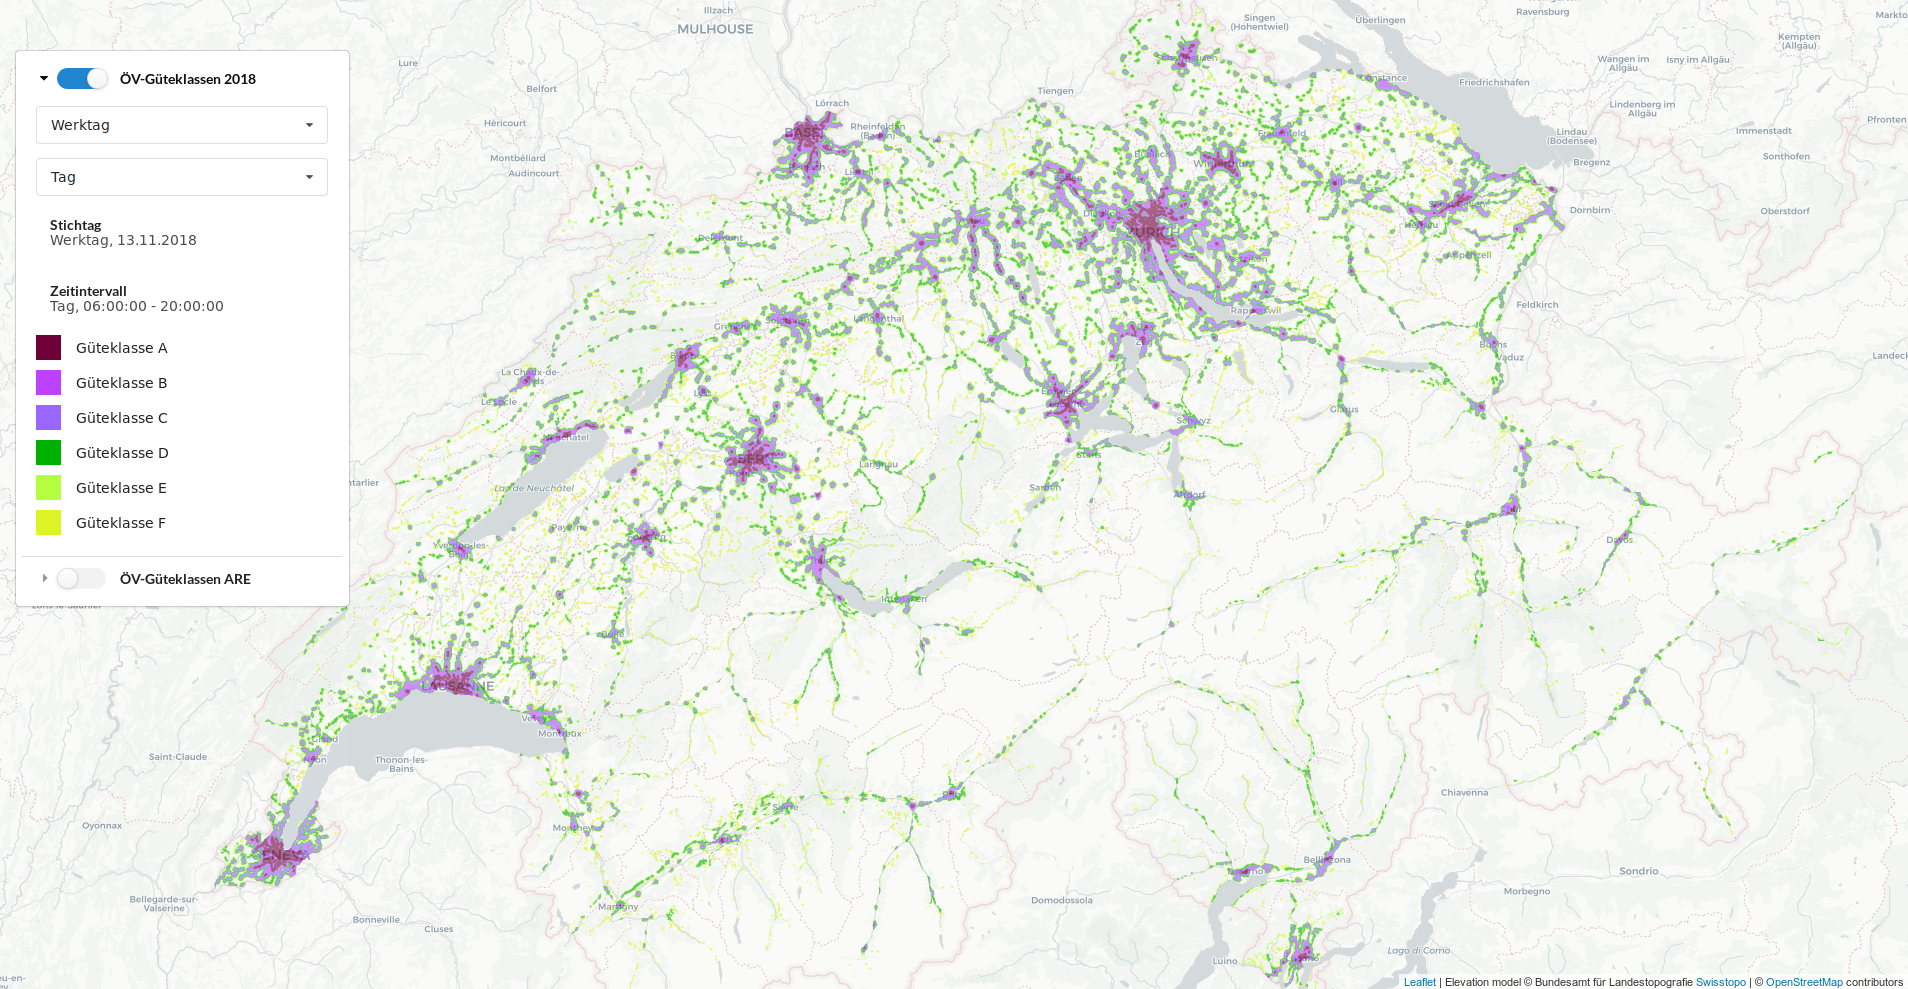
\includegraphics[width=1\linewidth]{technicalreport/img/resultat_oevgk18_uebersicht}
    \caption[Darstellung der berechneten ÖV-Güteklassen in der Web-Applikation]{Darstellung der berechneten ÖV-Güteklassen in der Web-Applikation}
    \label{fig:resultat_webapp_uebersicht}
\end{figure}
\end{landscape}

Zusätzlich zur automatisierten Berechnung wurde eine Web-Applikation entwickelt, die es ermöglicht, die berechneten \acs{ÖV}-Güteklassen im Browser darzustellen (siehe Abbildung \ref{fig:resultat_webapp_uebersicht}).
Ebenfalls wurden darin die bisherigen \acs{ÖV}-Güteklassen vom Bundesamt für Raumentwicklung (\acs{ARE}) integriert, was einen visuellen Vergleich der beiden Resultate erleichtert.

\subsection{Vergleich mit bisherigen ÖV-Güteklassen}
\label{Resultate:Vergleich mit bisherigen ÖV-Güteklassen}

Im Folgenden wird an einigen Beispielen gezeigt, wie die Resultate unserer Berechnung der "`\acs{ÖV}-Güteklassen 2018"' von bisherigen Methoden abweichen.
Als Vergleich werden dazu die \acs{ÖV}-Güteklassen von \ac{ARE} aus dem Jahre 2018~\cite{berechnung_are} verwendet.

\subsubsection{Einfluss der Wegführung}

\begin{figure}[ht]
    \centering
    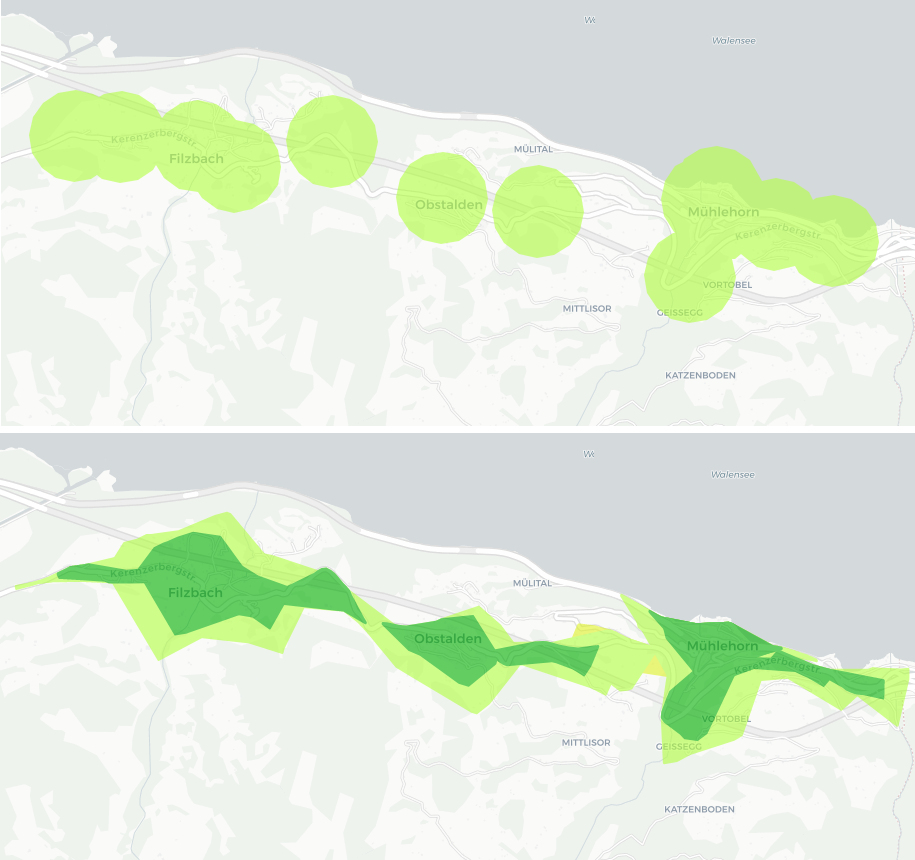
\includegraphics[width=0.8\linewidth]{technicalreport/img/vergleich_wegfuehrung}
    \caption[Vergleich zur Einfluss der Wegführung]{Vergleich zur Einfluss der Wegführung. Oben: ÖV-Güteklassen von \ac{ARE}. Unten: ÖV-Güteklassen 2018.}
    \label{fig:vergleich_wegfuehrung}
\end{figure}

Wie in \ref{Problemstellung:Luftlinie bei Einzugsgebieten} besprochen wird bei den bisherigen Ansätzen das Einzugsgebiet einer Haltestelle mit einem Kreis, und somit als Luftlinie, beschrieben.
Mit "`\acs{ÖV}-Güteklassen 2018"' wird nun das Einzugsgebiet durch eine \gls{Isochrone} beschrieben.
Die Fläche zeigt das Einzugsgebiet, das von einem Fussgänger von der Haltestelle aus in der definierten Zeit erreichbar ist.

Wie in Abbildung \ref{fig:vergleich_wegfuehrung} zu sehen ist, entstehen dadurch Geometrien, die dem Strassen- und Wegnetz folgen.
Dies ergibt einen realistischeren Eindruck über die effektiven Gebiete, die von einer Haltestelle erschlossen werden.

Die Berücksichtigung der Wegführung ist im Direktvergleich in Abbildung \ref{vergleich_wegfuehrung_are_isochrone} noch deutlicher sichtbar.

\begin{figure}[ht]
    \centering
    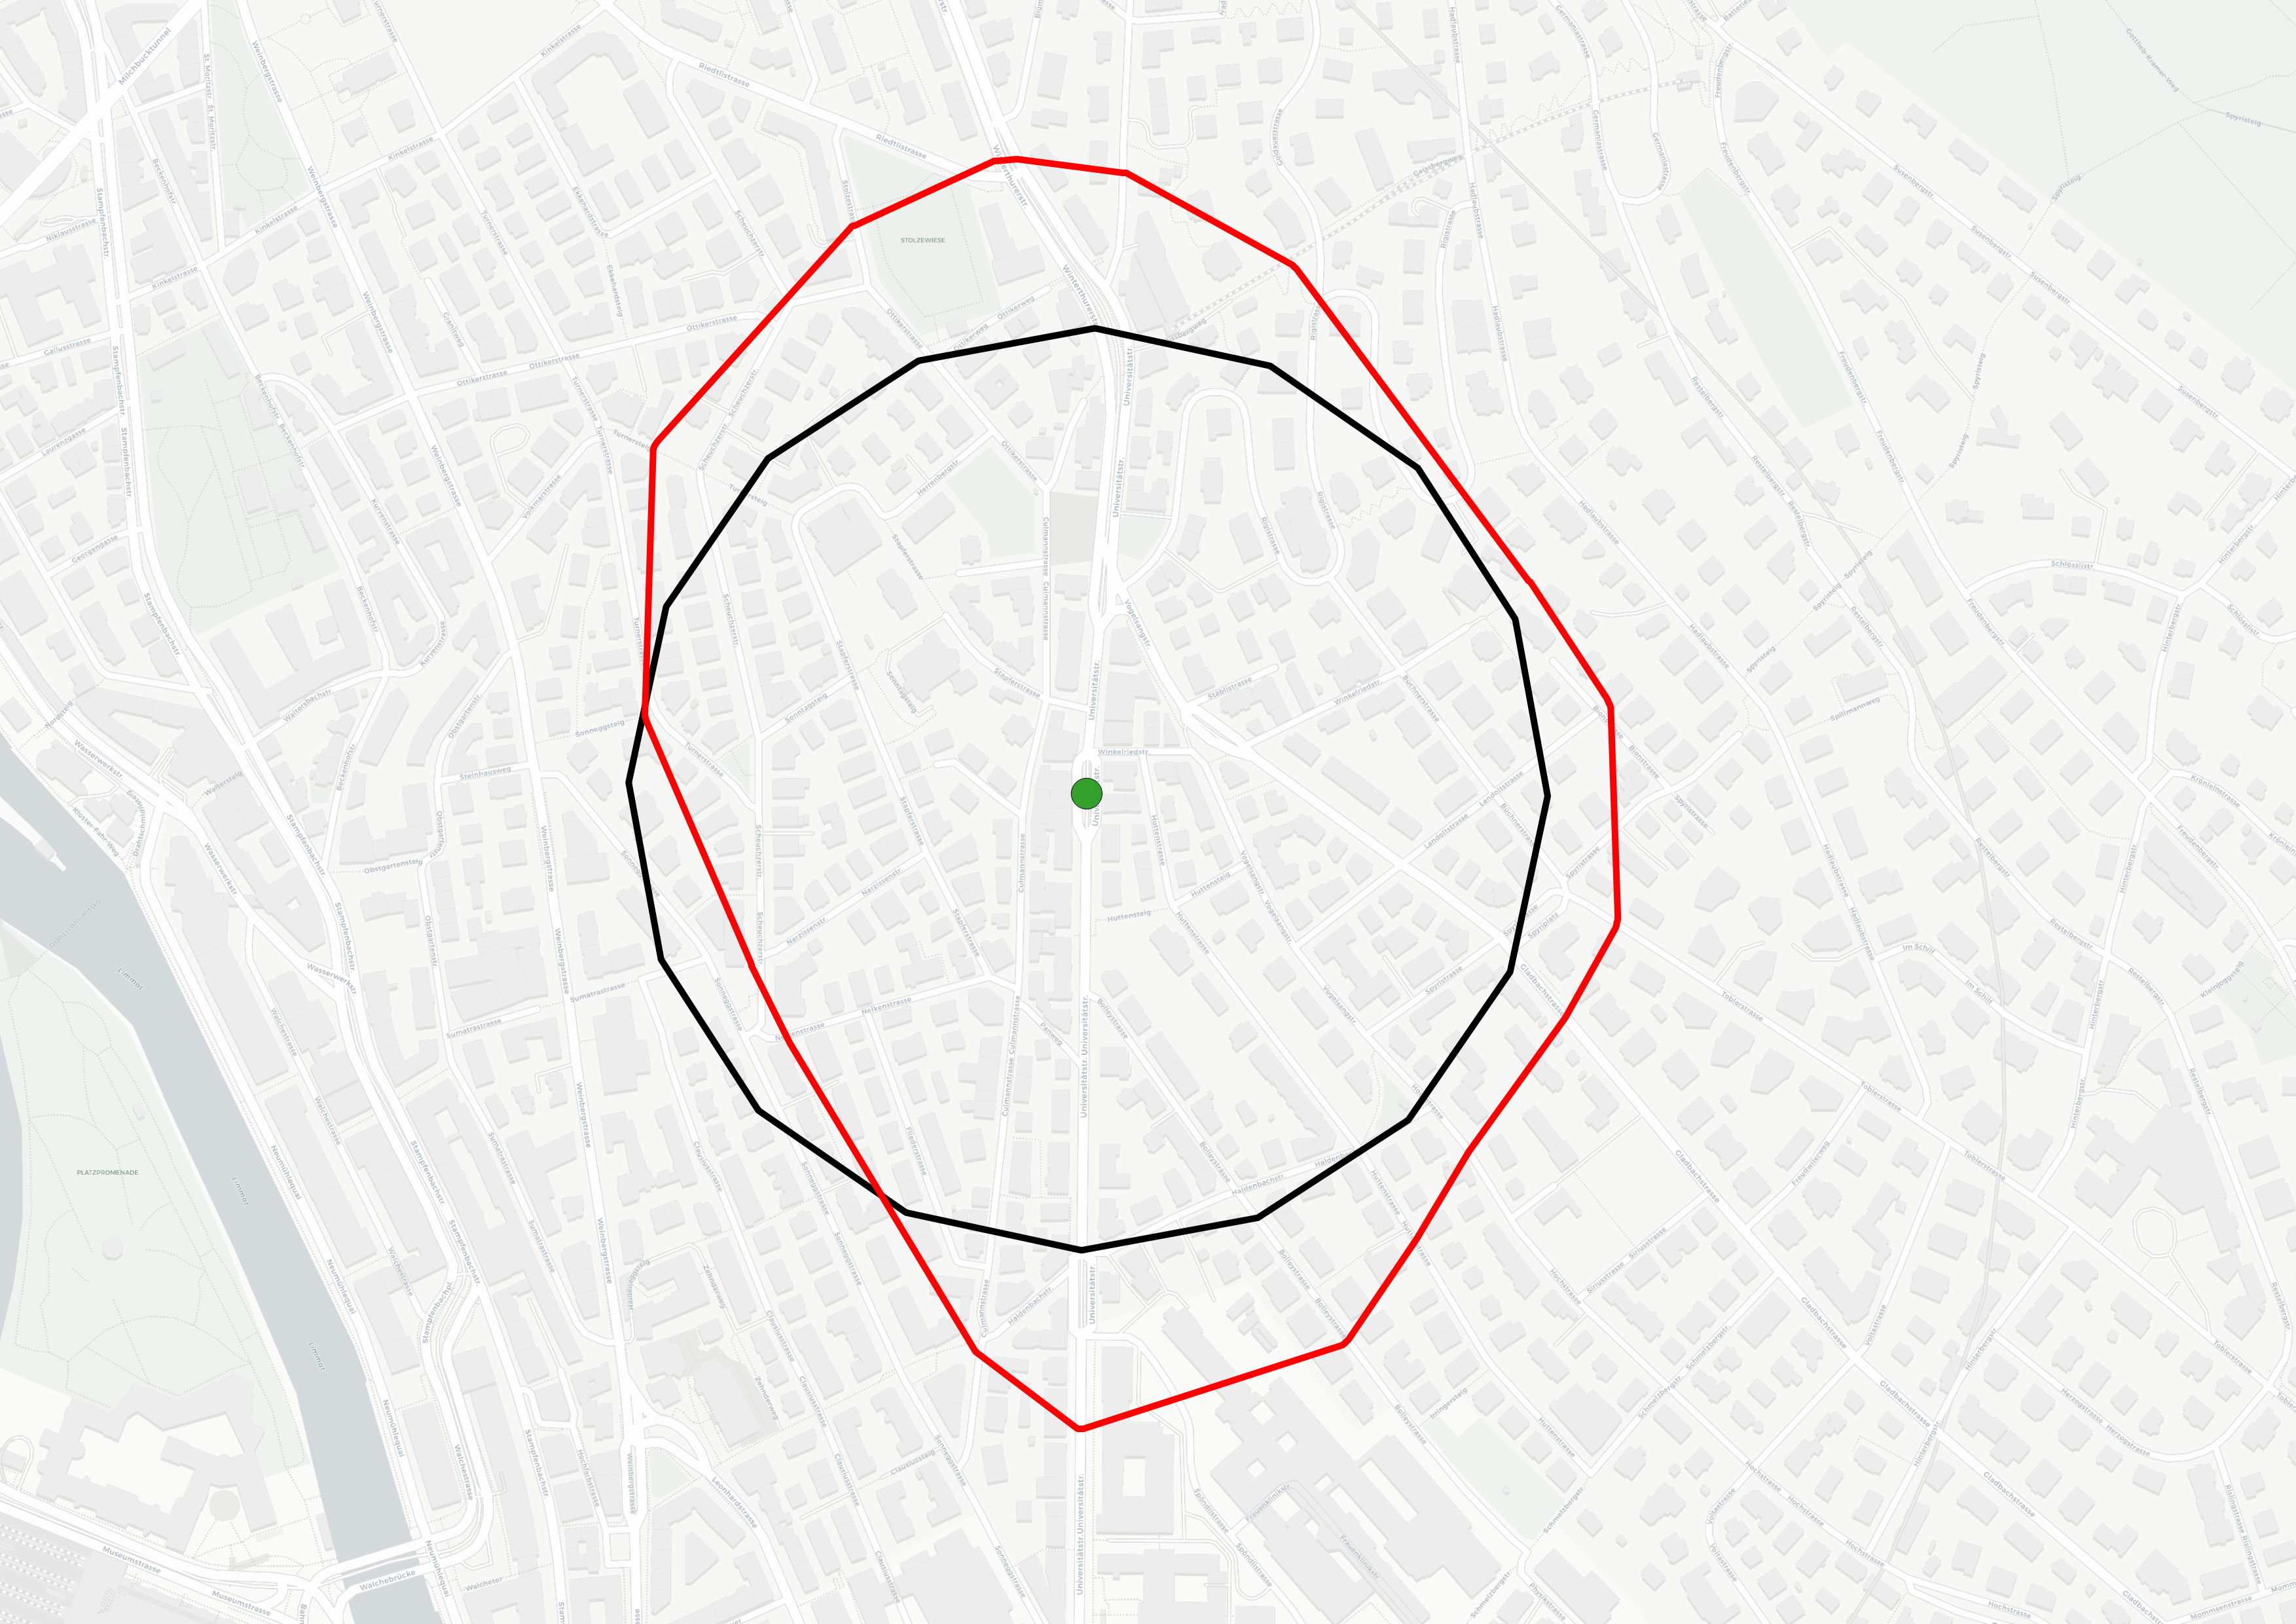
\includegraphics[width=0.8\linewidth]{technicalreport/img/vergleich_wegfuehrung_are_isochrone}
    \caption[Direktvergleich Einzugsgebiet ARE und Isochrone]{Direktvergleich Einzugsgebiet von ÖV-Güteklassen von \ac{ARE} (schwarz) und ÖV-Güteklassen 2018 (rot) ohne Berücksichtigung der Topografie; Zürich, Winkelriedstrasse}
    \label{fig:vergleich_wegfuehrung_are_isochrone}
\end{figure}

\subsubsection{Einfluss der Topografie}

Der Stand der Technik berücksichtigt die Topografie nicht konsequent.
Somit hat eine anspruchsvolle Topografie keinen Einfluss auf das Einzugsgebiet einer Haltestelle.
Das sieht man gut, wenn man die ÖV-Güteklasse des \acl{ARE} in Abbildung \ref{fig:vergleich_wegfuehrung_are_isochrone} betrachtet.
Auf der gut sichbaren Strecke (Universitätsstrasse) werden im Durchmesser des schwarzen Kreises über eine Distanz von 300 Metern 9 Höhenmetern zurückgelegt.
Nach der Definition der Berechnung der Leistungskilometern (siehe Kapitel \ref{Berechnungsmethodik OeVGK18:Gehzeit zur Haltestelle}) sind das zu den 300 Metern 90 Leistungsmeter, welche zurückgelegt werden müssen.
Der Einfluss der Topografie ist nun im Direktvergleich in Abbildung \ref{fig:vergleich_wegfuehrung_isochrone_mit_ohne_topo} sichtbar.
Die Haltestelle hat mit Einbezug der Topografie ein kleineres Einzugsgebiet.
Man sieht, dass sich dies gut im unteren Teil bemerktbar macht.
Die Strecke han von unten nach oben gesehen einen starken Anstieg, welche ins Gewicht fällt.
Beachtet man die Fläche von oben nach unten sieht man nur geringe Unterschiede, da das Gefälle den Grenzwert von 20\% nicht überschreitet.

\begin{figure}[ht]
    \centering
    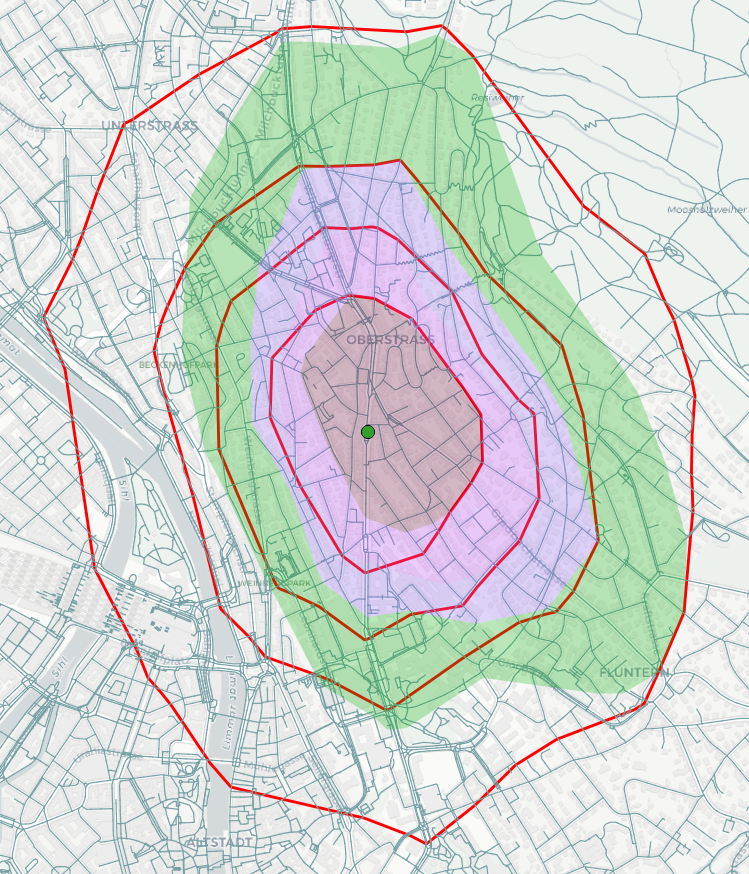
\includegraphics[width=0.8\linewidth]{technicalreport/img/vergleich_wegfuehrung_isochrone_mit_ohne_topo.png}
    \caption[Direktvergleich Einzugsgebiet Isochronen mit und ohne Topografie]{Direktvergleich Einzugsgebiet Isochronen mit (Fläche ausgefüllt) und ohne (rot) Berücksichtigung der Topografie; Zürich, Winkelriedstrasse}
    \label{fig:vergleich_wegfuehrung_isochrone_mit_ohne_topo}
\end{figure}


\subsubsection{Verbesserte Berechnung des Kursintervalls}

Der Unterschied in der Berechnung des Kursintervalls ist gut sichtbar, wenn man die Haltestelle "`Aarau, Buchenhof"' betrachtet.
Damit wir die Berechnungsmethodiken OeVGK18 und OeVGK93 vergleichen können, nehmen wir für die Auswertung von OeVGK18 der Stichtag 21.03.2018. Die Fahrplandaten des OeVGK93 stammen vom 21.03.2017.
Dieser Vergleich ist in diesem Zusammenhang zulässig, da beide einen Werktag repräsentieren und keine Änderung im Fahrplan erkannt wurde.
Ebenfalls sieht man für diese Haltestelle die Korrektur, welche das \ac{ARE} für Verbindungen vornimmt, welche nur in eine Richtung befahren werden.
So wird die Anzahl Verbindungen in diesem Fall verdoppelt, um sie anschliessend bei der Berechnung wieder zu halbieren.

An diesem Tag werden im Intervall 06:00 bis 20:00 Uhr 56 Fahrten an dieser Haltestelle registriert.
Folgt man der Berechnungslogik des Bundesamts für Raumentwicklung, erfolgt daraus folgender Intervall:
$ 840 / ((56 * 2) / 2) = 15 \text{min}$

Betrachtet man nun einen Auszug der Abfahrten in Tabelle \ref{table:Abfahrtszeiten Aarau, Buchenhof}, sieht man, dass beide Buslinien 4 Minuten versetzt alle 30 Minuten verkehren.
Die Aussage, dass man an dieser Haltestelle einen 15-Minuten-Takt hat, ist somit nicht ganz korrekt.
Kommt man um 06:10 Uhr an die Haltestelle, wartet man 23 Minuten auf die nächste Verbindung.

\begin{table}[H]
    \centering
    \begin{tabular}[c]{l l}
        \toprule
        \textbf{Abfahrtszeit}   & \textbf{Bus-Nr}\\
        \midrule
        06:03                   & 7\\
        06:07                   & 5\\
        06:33                   & 7\\
        06:37                   & 5\\
        07:03                   & 7\\
        07:07                   & 5\\
        07:33                   & 7\\
        07:37                   & 5\\
        \dots                   & \dots\\
        \bottomrule
    \end{tabular}
    \caption{Abfahrtszeiten Bus 5 und 7, Aarau, Buchenhof}
    \label{table:Abfahrtszeiten Aarau, Buchenhof}
\end{table}

Die neue Intervall-Berechnung gemäss Kapitel \ref{Berechnungsmethodik OeVGK18:Kursintervall} ergibt nun für die gleiche Haltestelle den Intervall 23.1 Minuten.
Der Unterschied macht sich in der Bestimmung der Haltestellenkategorie bemerkbar.
Da es sich bei dieser Haltestelle um eine Busstation handelt, fällt man nach der OeVGK18-Spezifikation von der Haltestellekategorie IV (OeVGK93) in die Kategorie V.

Abschliessend kann man sagen, dass 23.1 Minuten eine bessere Annäherung an den eigentlichen Kursintervall als die 30 Minuten, die vom \acs{ARE} berechnet wurde.
Dadurch wird das wahrgenommene Angebot an der Haltestelle besser wiederspiegelt.

\subsubsection{Verbesserte Ermittlung von Bahnknoten}
Bei der Ermittlung der Bahnknoten werden nun Haltestelle berücksichtigt, welche Verbindungen in 6 verschiedene Richtungen haben oder Zugang zu einer Fernverkehrsverbindung haben.
Aufgrund der Daten des \acl{ARE} nehmen wir an, dass bei der Berechnung der OeVGK93 nur Haltestelle als Bahnknoten identifiziert werden, welche mindestens drei verschiedene Richtungen bedienen.
Diese Annahme kommt zustande, wenn man für die Bahnknoten des OeVGK98 die Anzahl verschiedenen Richtungen mit unserer Implementation eruiert.
Dabei gibt es mit "`Genève-Aéroport"' einen Ausreiser, welcher nur eine Richtung anbietet.
Die Problematik ist in Kapitel \ref{Verbesserungsmöglichkeiten:Bestimmung der Bahnknoten} beschrieben.

Ein direkter Vergleich ist in Tabelle \ref{table:Vergleich Anzahl Bahnknoten} ersichtlich.

\begin{table}[H]
    \centering
    \begin{tabular}[c]{l l l}
        \toprule
        \textbf{}
                                & \textbf{OeVGK93}
                                & \textbf{OeVGK18}\\
        \midrule
        \textbf{Anzahl Bahnknoten}
                                & 150
                                & 106\\
        \bottomrule
    \end{tabular}
    \caption{Vergleich Anzahl Bahnknoten}
    \label{table:Vergleich Anzahl Bahnknoten}
\end{table}

Da wir mindesten doppelt so viele verschiedene Richtungen wie OeVGK93 verlangen, schränken wir so die Identifikation als Bahnknoten ein, was sich in der Anzahl identifizierten Bahnknoten bemerkbar macht.

\begin{table}[H]
    \centering
    \begin{tabular}[c]{l l l}
        \toprule
        \textbf{}
                                            & \textbf{Anzahl Bahnknoten}\\
        \midrule
        \textbf{OeVGK93 $\cap$ OeVGK18}       & 92\\
        \textbf{OeVGK93 $\setminus$ OeVGK18}  & 58\\
        \textbf{OeVGK18 $\setminus$ OeVGK93}  & 14\\
        \bottomrule
    \end{tabular}
    \caption{Unterschiede in der Identifikation der Bahnknoten}
    \label{table:Unterschiede in der Identifikation der Bahnknoten}
\end{table}

Das durch die höhere Anzahl verlangter verschiedener Richtungen eine kleinere Menge als Bahnknoten identifizierte Haltestellen resultiert, scheint logisch.
Tabelle \ref{table:Unterschiede in der Identifikation der Bahnknoten} nimmt die Unterschiede in den resultierenden Bahnknoten unter die Lupe.
Überraschend ist, dass die Bahnknoten, welche durch OeVGK18 identifiziert werden, nicht komplett in OeVGK93 vorkommen.
Es handelt sich um 14 Haltestellen, welche OeVGK18 im Unterschied zu OeVGK93 als Bahnknoten bestimmt werden.
Dabei handelt es sich unter diesen um 2 Haltestellen, welche eine Fernverkehrsverbindung haben und so als Bahnknoten gezählt werden.
Warum die restlichen 12 Haltestellen nicht ebenfalls als Bahnknoten identifiziert sind, entzieht sich unseren Kenntnissen.
Darunter fällt beispielsweise die Haltestelle Flüelen mit 9 verschiedenen Richtungen.

\subsection{Ausblick: Weiterentwicklung}
\label{Resultate:Ausblick: Weiterentwicklung}

Durch die neue Spezifikation und Web-Applikation ist die Grundlage für weitere und fortgeschrittene Auswertungen geschaffen.

Verknüpft man die neuen \acs{ÖV}-Güteklassen mit der Bevölkerungsdichte, ist es möglich, Verbesserungspotential für den \acs{ÖV} zu eruieren.
Dadurch wären Auswertungen analog zu "`95\% der wohnhaften Personen in einem bestimmten Gebiet müssen mindestens in der \acs{ÖV}-Güteklassen XYZ sein"' möglich.

Aber auch für den privaten Gebrauch ist eine Weiterentwicklung von Interesse.
So ist ein Wohnortfinder denkbar, welcher die Qualität des \acs{ÖV}-Anschlusses und anderen Faktoren (Nähe zu einer Schule oder Krankenhaus, etc.) berücksichtigt.

Für die Berechnung der Einzugsgebiete wird in dieser Arbeit der Ansatz von \glspl{Isochrone} verwendet, die entlang des Strassen- und Wegnetzes verlaufen.
Die Grundannahme dahinter ist, dass sich Fussgänger immer entlang des Wegnetzes fortbewegen.
Dabei gibt es Probleme bei offenen Fussgängerflächen, wie sie in~\cite{plaza_route} behandelt werden.
Ein anderer Ansatz basiert statt auf Routen auf einem Raster~\cite{pedestrian_accessibility_planning}. Dieser geht davon aus, dass sich Fussgänger überall fortbewegen, wo keine Hindernisse (Gebäude, Flüsse, Barrieren, etc.) sie daran hindern.
Dabei wird ein Raster über die Karte gelegt und jeder Kachel einen Kostenwert zugeordnet.
Für die Erzeugung der Einzugsgebiete werden dann vom Startpunkt aus in alle Richtungen die Kacheln eingefärbt und bei jedem Schritt die Kosten der Kachel addiert.
Dies wird so lange wiederholt, bis die gewünschten Maximalkosten erreicht werden.
In Abbildung \ref{fig:grid_based_approach} ist ein Ergebnis einer solchen Berechnung abgebildet.

\begin{figure}[ht]
    \centering
    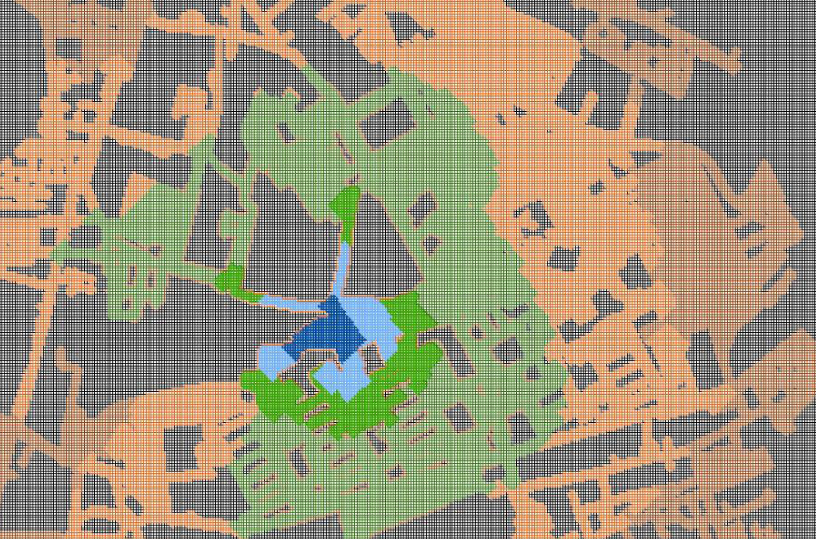
\includegraphics[width=0.6\linewidth]{start/img/grid_based_approach.png}
    \caption[Grid- beziehungsweise raster-basierter Ansatz]{Grid- beziehungsweise raster-basierter Ansatz~\cite{pedestrian_accessibility_planning}}
    \label{fig:grid_based_approach}
\end{figure}

Mit dieser Methode ist die Qualität des Routing-Graphen und Problematiken wie bei Fussgängerflächen weniger relevant.
Für die Berechnung von \acs{ÖV}-Güteklassen wäre dies ein spannender Ansatz für den Vergleich mit der Lösung in dieser Arbeit.

\subsection{Dank}
\label{Resultate:Dank}

Wir möchten folgenden Personen für ihre Unterstützung und Mitwirkung bei dieser Arbeit danken:

\textbf{Prof. Stefan Keller, IFS Institut für Software,} für die Zeit, Ressourcen, Kontakte, Know-How und Unterstützung, von welcher wir jederzeit profitieren konnten.

\textbf{Prof. Claudio Büchel, IRAP Institut für Raumentwicklung}, für die initiale Idee, Know-How über Verkehrsplanung und Fachunterstützung über das gesamte Projekt.

\textbf{Mitarbeiter, IFS Institut für Software,} für den regen Know-How-Austausch und die Unterstützung bei der Produktivsetzung.
